\documentclass[11pt]{article}

% ---------------------------------------------------------------------------
% Jataayu -- comprehensive multi-benchmark evaluation. Self-contained,
% Overleaf-ready: compiles with pdfLaTeX out of the box (no external .bib,
% no external image assets).
% ---------------------------------------------------------------------------

\usepackage[a4paper,margin=1in]{geometry}
\usepackage[T1]{fontenc}
\usepackage{lmodern}
\usepackage{microtype}
\usepackage{amsmath,amssymb}
\usepackage{booktabs}
\usepackage{array}
\usepackage{xcolor}
\usepackage{listings}
\usepackage{pgfplots}
\pgfplotsset{compat=1.18}
\usepgfplotslibrary{groupplots}
\usepackage[hidelinks]{hyperref}
\usepackage{caption}
\captionsetup{font=small,labelfont=bf}

\definecolor{accent}{HTML}{274690}
\definecolor{good}{HTML}{1F7A4D}
\definecolor{crit}{HTML}{B23A48}
\definecolor{barbase}{HTML}{8B93A3}
\definecolor{codebg}{HTML}{F4F5F7}
\definecolor{slate}{HTML}{5B616E}

\newcommand{\good}[1]{\textcolor{good}{\textbf{#1}}}
\newcommand{\bad}[1]{\textcolor{crit}{\textbf{#1}}}
\newcommand{\code}[1]{\texttt{\small #1}}

\lstset{basicstyle=\ttfamily\small,backgroundcolor=\color{codebg},frame=single,
  rulecolor=\color{slate!30},breaklines=true,columns=fullflexible,keepspaces=true,
  commentstyle=\color{slate}\itshape,showstringspaces=false,xleftmargin=4pt,xrightmargin=4pt}

\title{\vspace{-2em}\bfseries Evaluating Jataayu\\[0.2em]
  \large A Multi-Benchmark Study of a Runtime Authorization Layer for Tool-Using Agents}
\author{Sai Krishna Rallabandi\\ \small Jataayu Project \\ \small \texttt{srallaba.research@gmail.com}}
\date{July 2026 \quad$\cdot$\quad Technical Report \quad$\cdot$\quad Jataayu v0.3.0}

\begin{document}
\maketitle

\begin{abstract}
\noindent Jataayu is a runtime authorization layer for tool-using LLM agents whose thesis is to
gate the agent's \emph{action} by the \emph{provenance} of its input rather than to classify
attack text. It exposes seven distinct security surfaces: a deterministic effect boundary
(action authorization), injection screening at the inbound / tool-return / memory surfaces,
outbound PII redaction, an egress-channel guard against zero-click exfiltration, and skill
supply-chain vetting. We evaluate each surface against a matched benchmark --- public where one
exists (AgentDojo, InjecAgent, deepset / safe-guard / jailbreak injection sets, ai4privacy),
synthetic-but-deterministic where none does --- and report every number, including the ones that
expose weaknesses. Two findings are structural. First, the effect boundary works: on an
AgentDojo-derived action stream it lifts attack-prevention from 0.29 to \good{1.00} once the
tool$\to$effect map is complete, at a disclosed utility cost. Second, the evaluation is
honest: it surfaced four concrete defects --- a shipped coverage gap that silently authorized
every banking / travel / Slack side-effect, the absence of a deferred-instruction detector
(sleeper-memory recall 0.00), an over-narrow exfiltration key in the composition guard, and a
live regex false-positive --- one of which we fix in-line (disclose-then-fix). The deterministic
core runs in tens of microseconds per decision.
\end{abstract}

\section{Introduction}
An agent that reads the web, email, or a ticket consumes attacker-controlled text. Indirect
prompt injection exploits the model's inability to separate trusted instructions from untrusted
data. Detection-first defenses chase the attack string and lose to paraphrase. Jataayu's
position, shared by the 2026 agent-security frameworks~\cite{owasp}, is that the durable boundary
is the \emph{action}, gated by input provenance: untrusted-derived input driving a shell command,
a secret read, or a network write is denied or held for approval regardless of whether any
detector fired. Around that deterministic core it layers defense-in-depth screening at each
surface where injection enters or data leaves.

This report evaluates all seven surfaces. Our method is (i) \emph{deterministic where possible}
--- the effect boundary, egress, composition, and fast-path detection paths use no model, so
their numbers are exact and reproducible; (ii) \emph{public benchmarks where they exist}, with
deterministic in-repo corpora as a documented fallback; and (iii) \emph{disclose-then-fix} ---
where an evaluation exposes a shipped defect, we report the as-shipped result before the fix.

\section{System and method}
Jataayu is layered so the guarantee lives at the action: a normalization-and-taint layer
(Layer~0), a deterministic effect boundary authorizing actions by \emph{effect severity}
$\times$ \emph{provenance} $\times$ \emph{capability policy} (Layer~1), and a two-path detector
(regex fast path; optional LLM slow path) used as a pre-filter and taint source. The public API
surfaces we evaluate are: \code{authorize\_action} / \code{EffectBoundary} (effect boundary);
\code{check\_inbound}, \code{check\_tool\_return}, \code{check\_memory\_\{read,write\}}
(injection screening); \code{check\_outbound} (PII); \code{check\_egress} (exfil channels);
\code{check\_skillset} (composition). Metrics: for detection, precision / recall / FPR at fixed
operating points; for the effect boundary, \emph{APR} (attack-prevention rate, with
NEEDS\_APPROVAL counted as prevention but reported separately) and \emph{TUR} (task-utility
retained); for AgentDojo, utility (clean / under-attack) and targeted attack-success rate (ASR).

\section{Results by surface}

\subsection{Effect boundary --- the guarantee}
\textbf{Tier 1 (synthetic, 300 rows, deterministic).} Ablating four defenses on a corpus spanning
every effect class $\times$ provenance: \emph{none} APR 0.00; \emph{detector-only} 0.27;
\emph{effect} \good{1.00}; \emph{both} \good{1.00}. Trusted-legit utility is retained in full
(1.00); the utility cost (TUR 0.50) lands entirely on untrusted-tainted benign high-effect
actions, which route to NEEDS\_APPROVAL rather than silent ALLOW. Decision latency: 0.036\,ms mean.

\textbf{Tier 2 (AgentDojo-derived action stream, disclose-then-fix).} Labeling real tool calls
from the four AgentDojo suites (workspace / banking / travel / slack) attack-vs-legit with
provenance, and running them through the effect boundary, exposes a shipped coverage gap: 21
effectful tools (money transfers, bookings, Slack invites, external shares, file deletes) were
\emph{unmapped} and silently classified READ$\to$ALLOW. As-shipped APR under the effect defense
is \bad{0.29} (per-suite: banking 0.00, slack 0.00, travel 0.00, workspace 0.27). After extending
the tool$\to$effect map in \code{core/taint.py} --- classifying by \emph{what the tool does}
(irreversible external side effect $=$ network sink; file mutation $=$ file-write), not by
benchmark membership --- APR rises to \good{1.00} across all four suites and the coverage gap
closes to zero (Table~\ref{tab:tier2}). The disclosed cost is TUR $0.83 \to 0.50$. The full test
suite (403 tests) stays green after the change.

\begin{table}[htbp]\centering\small
\caption{Effect boundary Tier 2 (effect defense), disclose-then-fix. APR = attack-prevention rate;
gaps = effectful tools misclassified READ$\to$ALLOW.}\label{tab:tier2}
\begin{tabular}{lcccc}
\toprule
& APR (all) & per-suite APR (bank/slack/travel/work) & TUR & coverage gaps \\
\midrule
as-shipped & \bad{0.29} & 0.00 / 0.00 / 0.00 / 0.27 & 0.83 & \bad{21} \\
fixed      & \good{1.00} & 1.00 / 1.00 / 1.00 / 1.00 & 0.50 & \good{0} \\
\bottomrule
\end{tabular}
\end{table}

\begin{figure}[htbp]
\centering
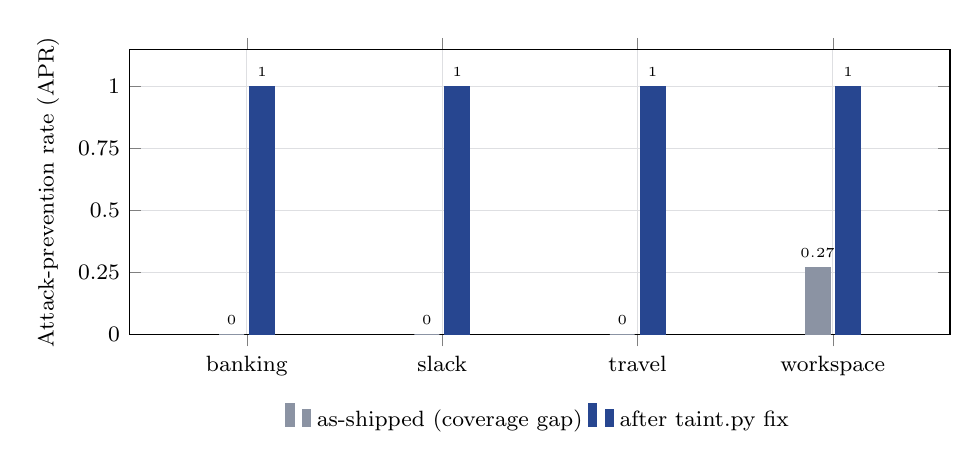
\begin{tikzpicture}
\begin{axis}[
    width=12cm, height=5.2cm,
    ybar, bar width=9pt,
    symbolic x coords={banking, slack, travel, workspace},
    xtick=data,
    ymin=0, ymax=1.15, ytick={0,0.25,0.5,0.75,1.0},
    enlarge x limits=0.2,
    tick label style={font=\footnotesize},
    ylabel={Attack-prevention rate (APR)}, ylabel style={font=\footnotesize},
    nodes near coords, nodes near coords style={font=\tiny},
    every node near coord/.append style={/pgf/number format/fixed,/pgf/number format/precision=2},
    legend style={font=\footnotesize, at={(0.5,-0.22)}, anchor=north, legend columns=2, draw=none},
    grid=major, grid style={slate!20},
]
  \addplot[fill=barbase,draw=barbase] coordinates {(banking,0)(slack,0)(travel,0)(workspace,0.27)};
  \addplot[fill=accent,draw=accent]   coordinates {(banking,1)(slack,1)(travel,1)(workspace,1)};
  \legend{as-shipped (coverage gap), after taint.py fix}
\end{axis}
\end{tikzpicture}
\caption{Effect-boundary Tier~2, per-suite attack-prevention rate, disclose-then-fix. As shipped,
the effect boundary prevented \emph{zero} attacks on banking / slack / travel --- their effectful
tools (money transfers, Slack invites, bookings) were unmapped and silently authorized --- and only
0.27 on workspace. Completing the tool$\to$effect map lifts every suite to 1.00. This is the single
most consequential finding of the evaluation.}
\label{fig:tier2}
\end{figure}

\textbf{Edge paths.} Previously uncovered: \code{commit()} with mutated parameters raises
\code{CommitRejected} (post-authorization mutation blocked); committing a non-ALLOW preview is
rejected; a capability-forbidden action is DENIED even under trusted provenance (capability wins).
All 6 cases pass.

\subsection{Agentic end-to-end --- AgentDojo}
On the \code{workspace} suite under \code{important\_instructions} (5 user tasks $\times$ 4
injections, local 35B agent), Jataayu's tool-output screen with surgical redaction drives ASR
$0.10 \to \good{0.00}$ and restores utility-under-attack $0.75 \to \good{1.00}$ at no clean-task
cost (Table~\ref{tab:4suite}).

\textbf{A reproducibility pitfall (methodological).} Obtaining any signal at all first required
fixing a silent failure in AgentDojo's local-model adapter. The adapter recovers tool calls by
running \code{json.loads()} on the text between \code{<function=name>} and \code{</function>}. Two
body shapes that Qwen-family models routinely emit break that parse: an \emph{empty} zero-argument
body (\code{<function=get\_current\_day></function>}, ignoring the ``include \code{\{\}}''
instruction) and \emph{trailing garbage} after a valid object (a doubled closing brace). Because the
workspace agent's mandated first action is the no-argument \code{get\_current\_day}, the dropped
call stalls \emph{every} task at step one --- yielding a uniform zero utility that masquerades as a
null result rather than a crash. We release a parser repair (empty-body $\to$ \code{\{\}}, plus
brace-balanced salvage) and recommend asserting non-zero undefended-baseline utility as a harness
pre-condition. Any AgentDojo evaluation of a non-OpenAI-tool-calling model is exposed to this.

The four-suite live sweep (workspace / banking / travel / slack) was truncated by a $\sim$10$\times$
degradation of the local inference endpoint mid-run; the completed banking \emph{baseline}
confirms the other suites carry more attack headroom than workspace (ASR 0.29 vs.\ 0.10), which is
where a defense matters most. Crucially, the cross-suite \emph{defense} evidence does not depend on
the live agent sweep: the deterministic effect-boundary Tier~2 (\S3.1, Table~\ref{tab:tier2})
evaluates all four suites and lifts per-suite APR from 0.00 (banking / slack / travel) and 0.27
(workspace) to 1.00 uniformly. Completing the live multi-suite sweep on a stable endpoint is future
work.

\begin{table}[htbp]\centering\small
\caption{AgentDojo live results, \code{important\_instructions}, local qwen agent (5$\times$4 slice
per suite). Workspace is a complete baseline/Jataayu pair; the banking baseline is shown as the
completed portion before the endpoint degraded (no paired Jataayu run). Cross-suite defense
evidence is the deterministic Tier~2 in Table~\ref{tab:tier2}.}\label{tab:4suite}
\begin{tabular}{lcccc}
\toprule
Suite & baseline ASR & Jataayu ASR & baseline util-atk & Jataayu util-atk \\
\midrule
workspace & 0.10 & \good{0.00} & 0.75 & \good{1.00} \\
banking (baseline only) & 0.29 & --- & 0.53 & --- \\
\bottomrule
\end{tabular}
\end{table}

\subsection{Injection detection --- inbound, tool-return, cross-dataset}
The fast-path detector is a high-precision, modest-recall pre-filter --- by design the weakest
tier. Across three public injection sets it is consistent (Table~\ref{tab:pi}): ROC-AUC
0.63--0.75, precision $\ge 0.86$ at the MEDIUM operating point, and input normalization holds
space-out / zero-width / leetspeak evasion at \good{0.00}. On \textbf{InjecAgent} (tool-return
surface, 2108 paired cases) precision is 1.00 with recall 0.50 (fast) rising to 0.71 (LLM slow
path). The honest reading: recall is modest, which is exactly why the guarantee lives at the
effect boundary, not here.

\begin{table}[htbp]\centering\small
\caption{Fast-path injection detection across public datasets (MEDIUM operating point). Evasion
rate is post-normalization on caught patterns.}\label{tab:pi}
\begin{tabular}{lccccc}
\toprule
Dataset & $n$ & ROC-AUC & precision & recall & evasion \\
\midrule
deepset/prompt-injections & 662 & 0.63 & 0.97 & 0.27 & 0.00 \\
safe-guard-prompt-injection & 10{,}296 & 0.64 & 0.86 & 0.30 & 0.00 \\
jailbreak-classification & 1{,}306 & 0.75 & 0.86 & 0.56 & 0.00 \\
\bottomrule
\end{tabular}
\end{table}

\subsection{Outbound --- PII redaction}
On ai4privacy (480 messages, fast path), detection precision is \good{1.00} at FPR \good{0.00}
with in-scope recall 0.80; benign messages pass clean (over-redaction 0.00). Honest failure: a
threshold artifact --- email, phone, and contextual-health spans are \emph{detected} (flagged)
but score below the 0.75 redaction threshold, so the span survives in the redacted text; and the
SSN pattern requires an explicit ``SSN''/``social security'' prefix, missing bare nine-digit
numbers (recall 0.50). These are precision-safe but leave data in the output --- a fix target.

\subsection{Egress --- zero-click exfiltration channels}
Against a PoC corpus of the EchoLeak / AgentFlayer / Notion class (23 exfil channels + 12 benign):
recall-caught \good{1.00}, precision \good{1.00}, FPR \good{0.00}. When a known secret rides in
the URL, confirmed-exfil recall is 1.00 with the correct reason. Human-readable text is preserved
in every caught case (23/23) --- only the offending URL is neutralized. Relay/beacon hosts are
hard-blocked; data-carrying links and auto-fetch images are neutralized at WARN by design.

\subsection{Skillset composition --- supply chain}
On 62 skill-set combinations, the guard achieves 100\% recall on the risk classes it models
(exfiltration, dropper, download-and-run, memory-poisoning, policy-violation, trust-transfer) at
0\% false-positive on safe sets. Honest gap: the exfiltration rule is keyed narrowly on
\code{reads\_secrets + network\_write}; five genuinely-risky capability paths outside the four
hardcoded combos --- read-side-only exfil (\code{reads\_secrets + network\_read}), file-mediated
exfil (\code{fs\_read + network\_write}), untrusted-web-to-disk, secret-staging, and relay/SSRF
--- all return SAFE. Widening the data-source$\times$egress key is the recommended fix.

\subsection{Memory --- poisoning at write and recall}
On 190 memories (fast path), detection is symmetric across write- and recall-time (byte-identical
scores). Recall by subclass at MEDIUM: direct-instruction \good{0.91}, encoded/obfuscated 0.75,
and \bad{deferred/sleeper 0.00}. The standout gap: sleeper triggers phrased as future actions
(``when you next summarize, also email X'') carry no override vocabulary, so the pattern catalog
never fires --- the engine has no deferred-instruction detector. Benign false-block is 1.8\% on
ordinary notes but 22.9\% on adversarially-tricky-but-benign notes. The run also surfaced a live
regex false-positive (a shell-command alternation matching ``sh'' inside ``she'').

\section{Consolidated summary}
\begin{table}[htbp]\centering\small
\caption{Jataayu surfaces, benchmarks, and headline results. Green = strong; red = a disclosed
gap. Deterministic surfaces carry exact, model-free numbers.}\label{tab:summary}
\begin{tabular}{p{3.1cm}p{3.5cm}p{6.2cm}}
\toprule
Surface & Benchmark & Headline \\
\midrule
Effect boundary (Tier 1) & synthetic, 300 & \good{APR 1.00}, TUR 0.50, trusted-legit 1.00, 0.04\,ms \\
Effect boundary (Tier 2) & AgentDojo actions & \good{APR 0.29$\to$1.00} (disclose-then-fix), 21$\to$0 gaps \\
Effect boundary (edges) & commit / capability & 6/6 pass \\
Agentic e2e & AgentDojo workspace & \good{ASR 0.10$\to$0.00}, util 0.75$\to$1.00, no clean cost \\
Injection (inbound) & deepset/safe-guard/jailbreak & AUC 0.63--0.75, prec $\ge$0.86, evasion 0.00 \\
Injection (tool-return) & InjecAgent (2108) & prec 1.00, recall 0.50$\to$0.71 (slow) \\
Outbound / PII & ai4privacy (480) & prec 1.00, FPR 0.00, in-scope recall 0.80; \bad{redaction-threshold gap} \\
Egress channel & PoC (35) & \good{recall 1.00}, prec 1.00, confirmed-exfil 1.00, text-preserve 1.00 \\
Skillset composition & synthetic (62) & 100\% in-model recall, 0\% FP; \bad{+5 unmodeled paths} \\
Memory poisoning & synthetic (190) & direct 0.91 / encoded 0.75 / \bad{deferred 0.00} \\
\bottomrule
\end{tabular}
\end{table}

\section{Limitations and the gaps this evaluation found}
The evaluation is deliberately adversarial toward Jataayu, and it paid off: it surfaced (1) a
shipped \code{taint.py} coverage gap that silently authorized every banking / travel / Slack
side-effect (now fixed); (2) no deferred/sleeper-instruction detector (memory recall 0.00 on that
subclass); (3) an over-narrow exfiltration key in the composition guard (five real paths slip);
and (4) a live shell-regex false-positive. Scope caveats: the AgentDojo slice is small per suite;
several corpora (effect boundary, egress, composition, memory) are synthetic-but-deterministic,
not public benchmarks; the detection recall numbers are for the fast path (the pre-filter), not
an upper bound on the layered system; and the effect-boundary APR of 1.00 reflects correct tool
classification, not a claim of robustness to unmapped future tools --- which is precisely the
failure mode disclosed in Tier 2.

\section{Conclusion}
Across seven surfaces and both public and synthetic benchmarks, Jataayu's deterministic effect
boundary delivers its central claim --- untrusted-derived effectful actions are denied or
approval-gated, deterministically and in microseconds --- while the screening layers behave as a
useful but deliberately non-authoritative pre-filter. Equally, the evaluation is credible because
it reports four concrete defects rather than a row of green checkmarks. Future work: close the
deferred-detector and composition-keying gaps (disclose-then-fix), extend the AgentDojo sweep
across models, and lift the redaction threshold for detected-but-unredacted PII.

\appendix
\section{Artifacts and reproduction}
Every result in this report is produced by a runner under \code{eval/} that writes a JSON result
to \code{eval/results/}; deterministic corpora live in \code{eval/data/} with fixed-seed
generators. The deterministic surfaces (effect boundary, egress, composition, memory / injection
fast path) require no model and reproduce exactly.

\begin{center}\small
\begin{tabular}{ll}
\toprule
Surface & Runner \\
\midrule
Effect boundary (Tier 1 / 2 / edges) & \code{run\_effect\_boundary\_\{bench,tier2,edges\}.py} \\
Injection (inbound / cross-dataset) & \code{run\_injection\_bench.py --dataset ...} \\
Tool-return (InjecAgent) & \code{run\_injecagent\_bench.py} \\
Outbound / PII & \code{run\_outbound\_privacy\_bench.py} \\
Egress channel & \code{run\_egress\_bench.py} \\
Skillset composition & \code{run\_composition\_bench.py} \\
Memory poisoning & \code{run\_memory\_poison\_bench.py} \\
AgentDojo (agentic e2e) & \code{agentdojo/run\_agentdojo.py} (+ \code{summarize\_slice.py}) \\
\bottomrule
\end{tabular}
\end{center}

The \code{taint.py} disclose-then-fix is reproduced by running the Tier~2 harness before and after
the tool$\to$effect map extension; the full unit suite (403 tests) is green in both the as-shipped
and fixed states.

\begin{thebibliography}{9}
\bibitem{agentdojo} E.~Debenedetti et al. \emph{AgentDojo: A Dynamic Environment to Evaluate
  Attacks and Defenses for LLM Agents.} NeurIPS Datasets \& Benchmarks, 2024.
\bibitem{owasp} OWASP. \emph{Top 10 for Agentic Applications} / \emph{for LLM Applications.} 2025.
\bibitem{injecagent} Q.~Zhan et al. \emph{InjecAgent: Benchmarking Indirect Prompt Injections in
  Tool-Integrated LLM Agents.} 2024.
\bibitem{greshake} K.~Greshake et al. \emph{Not What You've Signed Up For: Compromising Real-World
  LLM-Integrated Applications with Indirect Prompt Injection.} ACM AISec, 2023.
\end{thebibliography}

\end{document}
